\chapter{Protein Structure}
\section{Protein Structure - Lecture 4}

\subsection*{The Classical Structure-Function Paradigm}
\begin{figure}[h!]
    \centering
    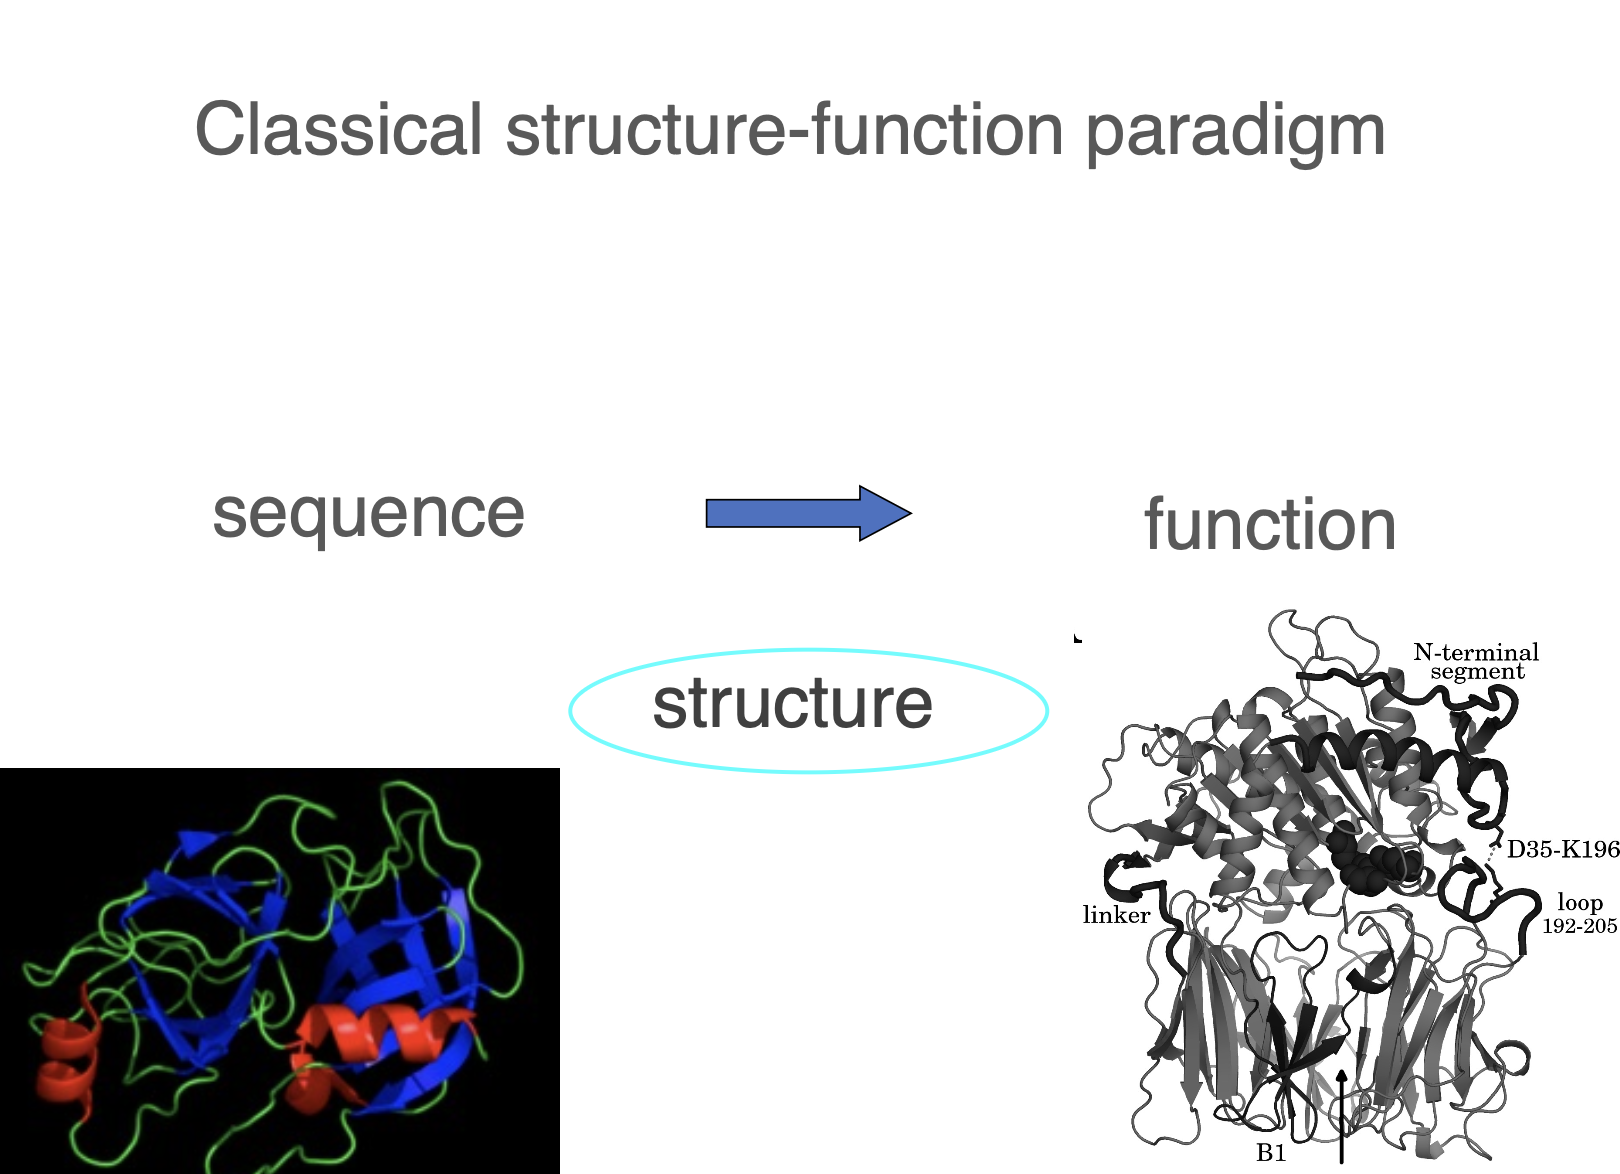
\includegraphics[width =0.8\linewidth]{slides/protein_structure/classical_structure_function_paradigm.png}
    \caption*{}
    \label{fig:placeholder}
\end{figure}

\noindent People work with this. It's called a classical structure-function paradigm, and they believe that the protein sequence encodes the function through a well-defined structure of a protein. What you need to see as a physicist is that this is a \textbf{deterministic relationship without any uncertainties}. This is what biologists believe in, this is what chemists believe in, and this had been a very strong constraint on the whole field of biology, and this is what gives you opportunity to work in the coming decades and a good salary or gain good research reputation, whatsoever. \textbf{The fact that this is not true.} This is your future. What you need to understand, again as a physicist, that this is a deterministic relationship making no notions whatsoever things that, for example, these entities, sequence, function or structure, can be \textbf{ensembles}. 


\subsection*{Learn how to read sequences}
\begin{figure}[h!]
    \centering
    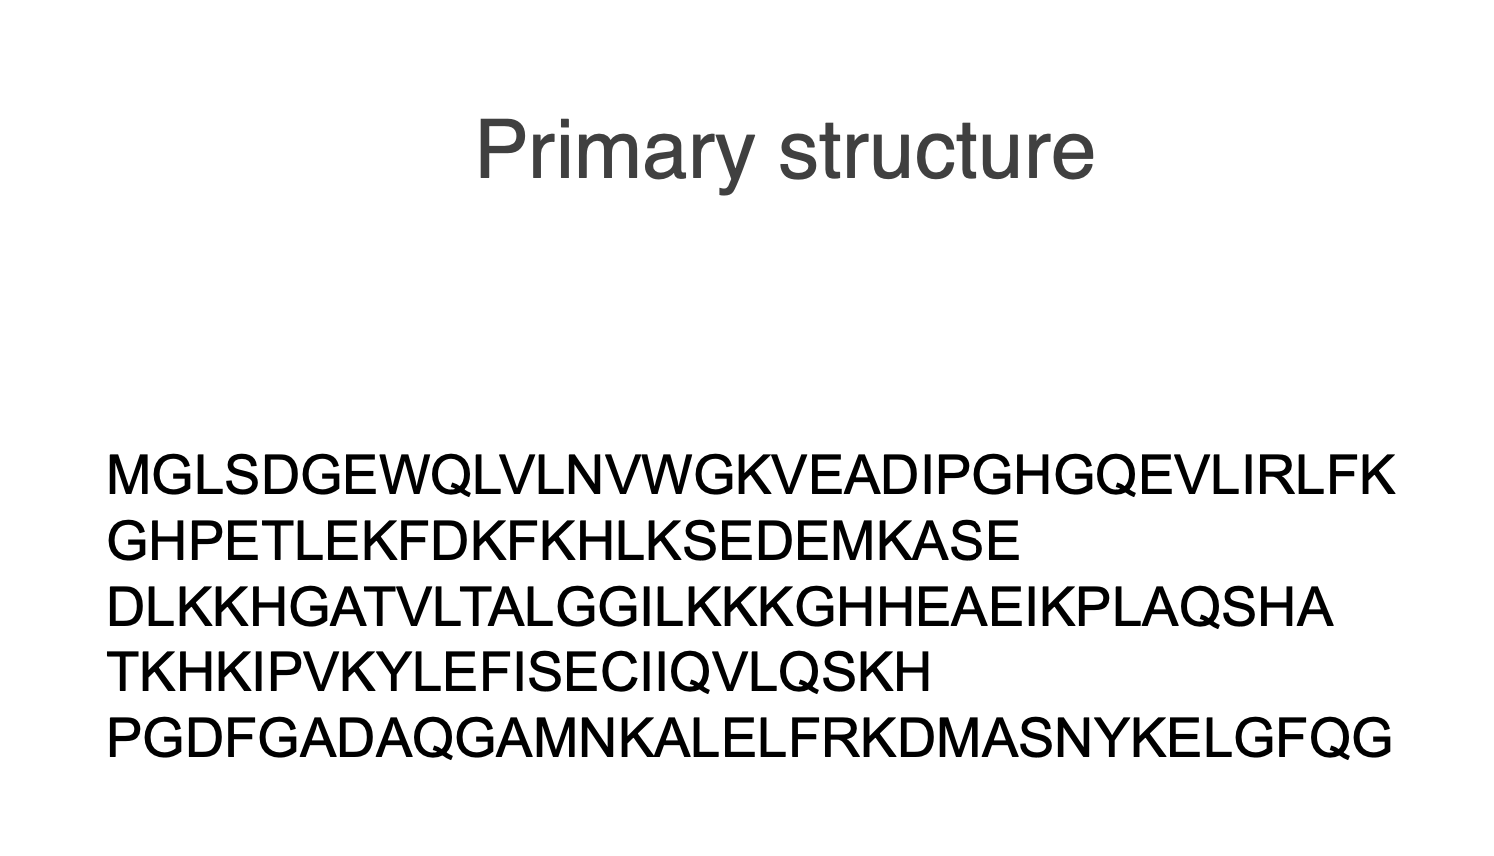
\includegraphics[width =0.8\linewidth]{slides/protein_structure/PRIMARY_STRUCTURE.png}
    \caption*{}
    \label{fig:placeholder}
\end{figure}
Let's start with the primary structure. \textbf{The very first thing I suggest you to do is to learn what the letters mean.}  Because you need to read it. Try to read it with your, I mean, with your intuition, nd try to note something. Believe me or not, I'm working with proteins kind of every day, and I am reading these. And sometimes from my own reading understand something, because why? Because the brain does some kind of well, intelligence. So, let me help you, let me teach you to read. 
\smallskip \newline \noindent
If you look the whole text, do you find more or less the 20 letters? I mean, just as a first sight. Yeah, I mean, there is quite a bit of variations, maybe you don't need to there is quite a bit of variation in the letters. This we can say. Then, you know, if I start reading it, there is one follows another, so it's not the same letter. So, it's there are different letters. And then you keep reading, and then you let's say arrive at this line, you say KK and GG and KKK, even three the same. So, there are some things which are kind of repetitive. 

\subsection*{The Aminoacids}
\begin{figure}[h!]
    \centering
    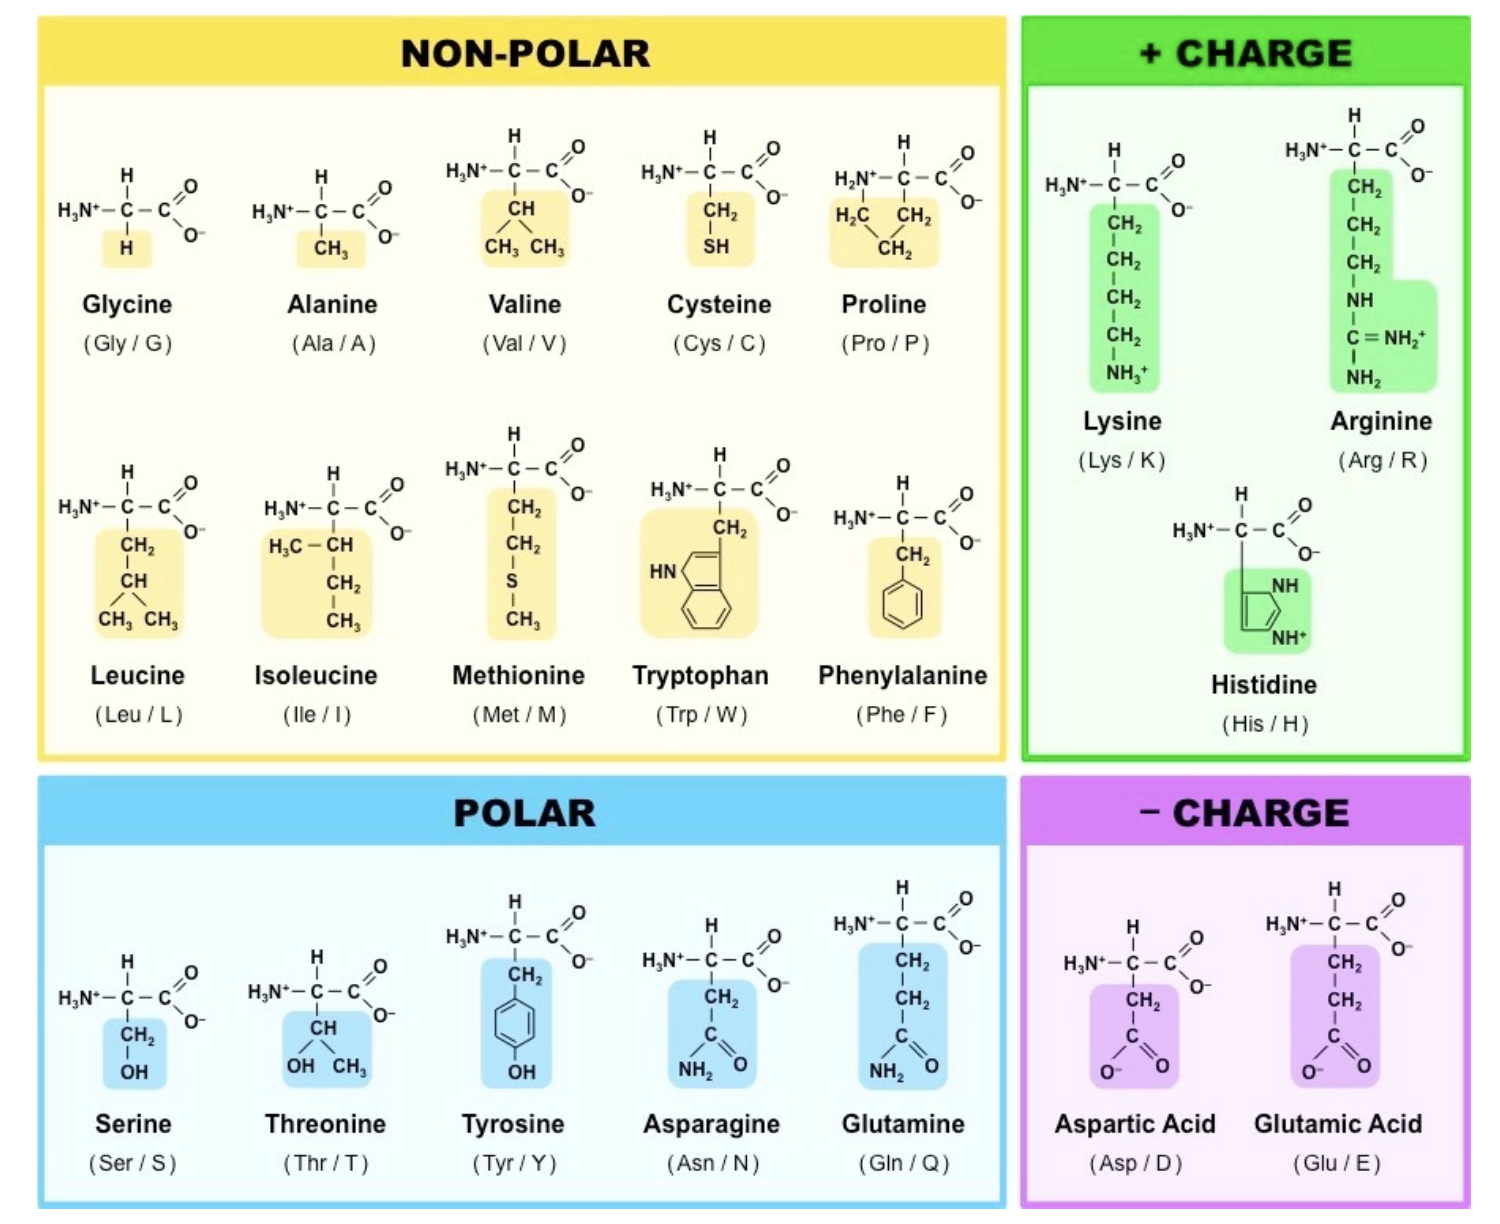
\includegraphics[width =\linewidth]{slides/protein_structure/aminoacid_table.png}
    \caption*{}
    \label{fig:placeholder}
\end{figure}
So, we have 20. All the 20 have different properties. Now, this  picture  I suggest you to print out and put above your tables when if you really start doing some biological calculations. 
\paragraph{Polar and Non-Polar}
You see here words non-polar and polar. This means polar ones like water, non-polar ones don't like water, they prefer oil. I will only speak about very simple things and keep yourself simple even to do the best machine learning in the world. Okay? You don't have to be complicated, you just have to be clever.

You see that you have lots of non-polar I mean, if you just again, briefly look at the numbers, you the the largest group is the non-polar. \textbf{Why?}

 So, at the end of the day, we construct proteins that are several hundred residues, let's say. Most of them are compact. So, we have to get them compact. We construct them in a water-like environment. So, we have to make them compact. Now, if we put all the polar and later on charge, I they like water so they don't want to be compact simply. 

\paragraph{Protein Charge depends on pH}
We say charged, but it depends on which solution they are or which protein they are. I mean if you put the pH very high, then, you know, everything will be deprotonated. If you put the pH very low, then everything will be protonated. So, you know, it depends. So we can say it's charged, but when you compute machine learning, you have to put one number at that pH or at that protein or at the cytosol or somewhere. So this is not an absolute quantity, this is what I'm trying to tell you. 

\subsection*{Useful Properties of some Aminoacids}

I'm trying to call your attention to some properties that you may pick up when you do the machine learning. All amino acids are very special,we have to pick up their speciality, and understand if it's relevant to the problem that we are studying.


\begin{figure}[h!]
    \centering
    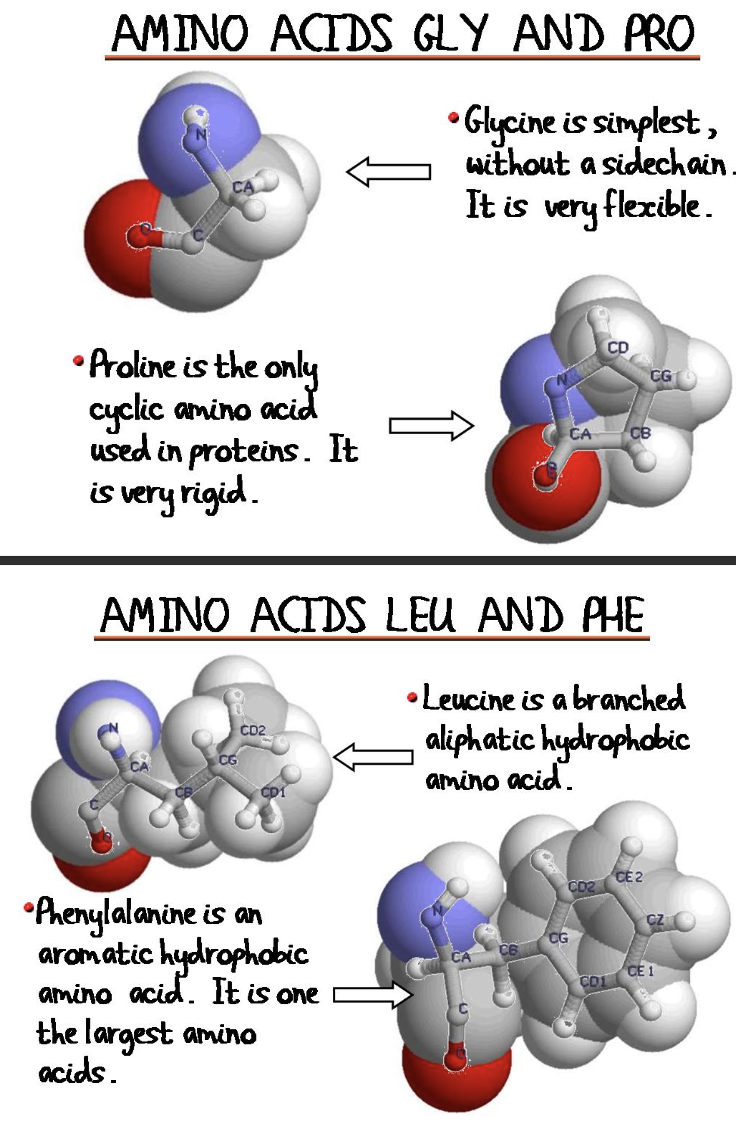
\includegraphics[width =0.48\linewidth]{slides/protein_structure/gly_pro.png}
    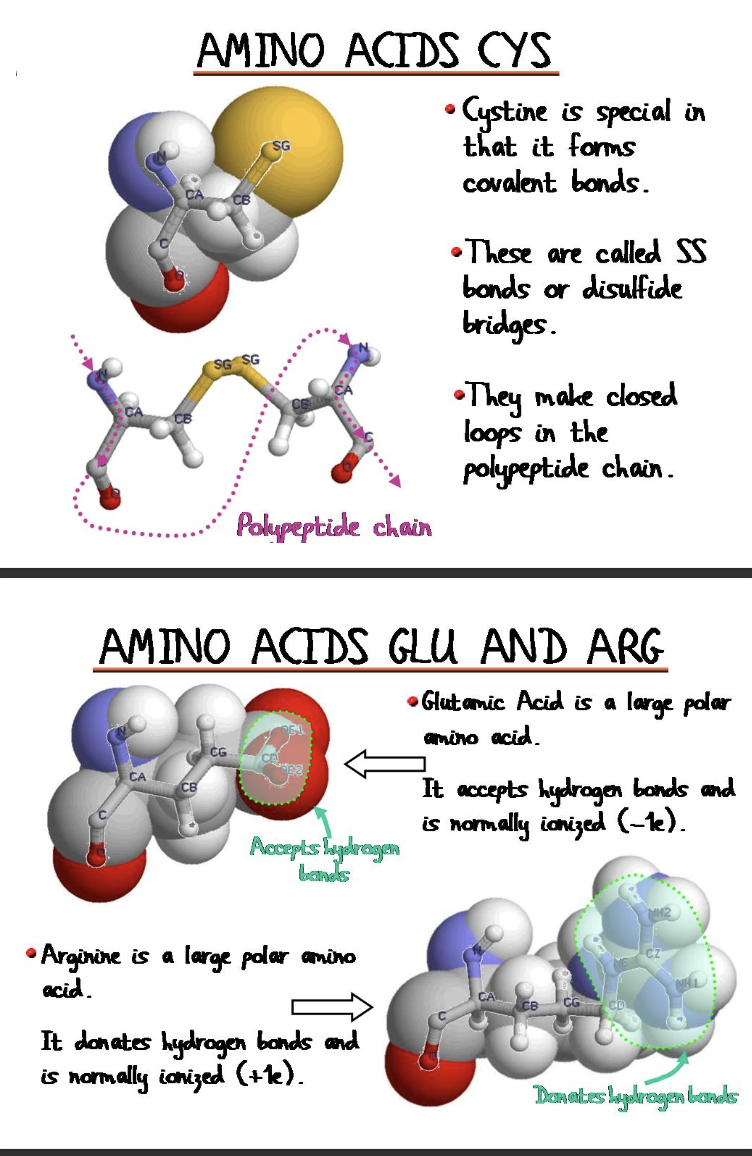
\includegraphics[width =0.48\linewidth]{slides/protein_structure/cys_arg.png}    
    \caption*{}
    \label{fig:placeholder}
\end{figure}


\paragraph{Glicine}
"So glycine, you see it's the C alpha, so that's the main chain, and here would be the side chain. Uh, and you see here two hydrogens. By the way, I explain you later these big balls represent the kind of the real atomic radius that we derived from electron diffraction. Okay? This is just to give you an idea, something which is very important: the volume, the space that the actual amino acid occupies. This will be important for later discussions. Okay? So this is what you see and this is kind of the skeleton."
So getting back to this, here we have two hydrogens. Okay? And these are the same. Now, this is chemically very special because normally you have a hydrogen here and something else, so the carbon atom here have four different substituents, and that has a—that has a consequence. \textbf{The first consequence is that when you have two small hydrogens, it will be very mobile. The second consequence is that because two atoms are the same, it cannot be chiral.} So there are two very important things. You can say: okay, but, you know, what to do, why I use in my language? For example, I tell you, when you learn more a bit about the biology or, you know, you select such problem; for example, if you learn about transcription, transcription is a super dynamical process. The enzymes that are doing it must have some tails, some parts that are full of glycines because it must be very flexible. 


\paragraph{Proline}
Then we have proline here. Now, proline is also very special. There is a covalent bond between the end of the side chain and the main chain. Now, this is a kind of—this is the only one where it's the case. Chemically actually it's called an imino acid, it's not even an amino acid, but this question we ask only from the medical students if you want them to fail the exam.
But what is important for you is that this is a big constraint. I mean you, you know, if you tighten the side chain to the main chain, and this limits—I mean there is some—we explain later about conformations and so on—this somehow limits the conformations and basically it will restrict \textbf{proline to two main states}. So things that want to change their function in a kind of binary manner would use proline because once in this state, once in the other state, only because of that constraint. 

\paragraph{Cystine - Dsulfide bridges}
 I take another amino acid—I won't go all through the twenty, I'm just giving you flavors. I take another which is called cysteine and cy—normally most of the side chains, if you look carefully, have a carbon, have oxygen, and nitrogen, these three. And hydrogens, of course. \textbf{This one also has a sulfur}. Big—first of all, you can see it's big, bigger than the others. Otherwise, there is another amino acid which is about the same size just there is oxygen here. Why it's interesting to have the sulfur? But the sulfur is a very sensitive atom in a sense that it can be SH if it's red—if it's reduced, and it can be SS—I mean S, okay, sulfur bound to sulfur, SS doesn't have a good notation, so sulfur bound covalently to a sulfur if the conditions are oxidizing. Having said that, since this is, you know, on one part of the main chain, maybe, you know, the other is on a completely different part of the main chain, through this kind of bonds, which are covalent bonds again, formed only if the conditions are proper, you can put a strain. When you form a covalent bond, you make a strain. You put a strain on the whole protein, you stabilize it, and many cases you have the situation when—I mean you—you have a protein, you know, something, and you cut it, actually it's happening in your stomach for example. You cut, but it doesn't fall apart because there is this kind of bond. Before this kind of bond is formed, and then you can cut the chain. Don't let's not go into the details why you cut the chain, but I'm just saying that this is the particular amino acid that can help to make such kind of connections that can help to stabilize under some conditions when conditions are oxidizing and it can form a bond with another of these. 


\paragraph{Phenylanine}
Then there are other amino acids, okay, leucine and phenylalanine, let's start with this one because this is easier. You can see that there is a ring here, but the ring is not connected to the main chain—this is the main chain. It's not connected, it's kind of free. You can see that there are six members and the particular feature of those six is that they are \textbf{planar}. And there are—I mean in classic—when you learn organic chemistry you draw like this—there are delocalized electrons. You can make of course a sandwich, this is you can suspect that this is an energetically favored, but the other is a T-conformation, this is energetically favored. And if you do calculations, actually in this case you can have one here and another on the other side—I don't have more hands, but you can imagine. This—this means that here you can very easily generate multiple states in a very easy manner. Okay, let's put it that way. This again, this super simple property expresses in itself in organizing protein assemblies, for example, in the very first lesson I showed you this \textbf{condensate}, this green dots in a cell, and I will show many—that's a key feature. 
\paragraph{Leucine}
You see the leucine, it's—it's all carbon and hydrogen. We say also hydrophobic, non-polar, just to get to know the words. Okay? And we say branched, because here there is a branch. Okay? Uh, why it's important? \textbf{Well, when it's branched, I mean it can occupy more space, and there can be more water released to the bulk, this kind of things.}
\paragraph{Glutamic Acid}
There is another residue which is negatively charged, which is one carbon less, so only this one and the carboxylate group comes immediately, that is called aspartate. You can ask immediately, why nature created two which are more or less the same? Not the same, because one can be protonated at a pH of four point three and the other at three point nine. This is aspartate and this is glutamate. They—it absolutely sets them for different enzymatic reactions. Nature played a lot in which cases uses glutamate, which cases uses aspartate. They many times participate in we call proton shuttling: they get a proton, get neutral, give up a proton, and so on. So that's an interesting property. 
\paragraph{Arginine}
Then we have positively charged residues, which are very different from one another, one is lysine—you can go back, this is just a very long chain with a positive charge at the end—and then we have this very exciting one which we call—is called arginine. And you see here this group is called in chemistry guanidium group. Now, the group names you don't need to know, but sometimes I can't avoid using the names. Okay? You see that there are three nitrogens here, center in the center there is a carbon, and the whole thing you may imagine as here it's—it's planar. Again, it's full of delocalized electrons. 
For a long time, many decades, we just considered arginine as, you know, one of the positively charged residues, it didn't really want to give up its positive charge, so it’s—you know, we didn't care that much about arginine. And suddenly, like ten years ago, more or less ten years ago, we got interested in arginine. Why? Because people discovered—I mean it's—it’s stupid—but people discovered that arginine has this delocalized electrons, and similarly what I explained about phenylalanine, it can make the sandwich, it can make the T-conformation. And what they realized first it was from machine learning, that this arginine is very important to form the protein condensates, this droplets in the cell. But they didn't understand why. So they had to go back to elementary chemistry. I—so it was first came out from machine learning really, published big journals, you know: the arginine is important. Do you remember about this protein condensates or shall I look for a video? What they—maybe I should, because I see some eyes that are not convincing for me. But I need glasses. One second, okay, I—I show you. I—I don't remember if it was a video of yours, but let—let—one second, okay, let me open one of my presentations and then you will—"

\subsection*{Amino-acid Classification}
\begin{figure}[h!]
    \centering
    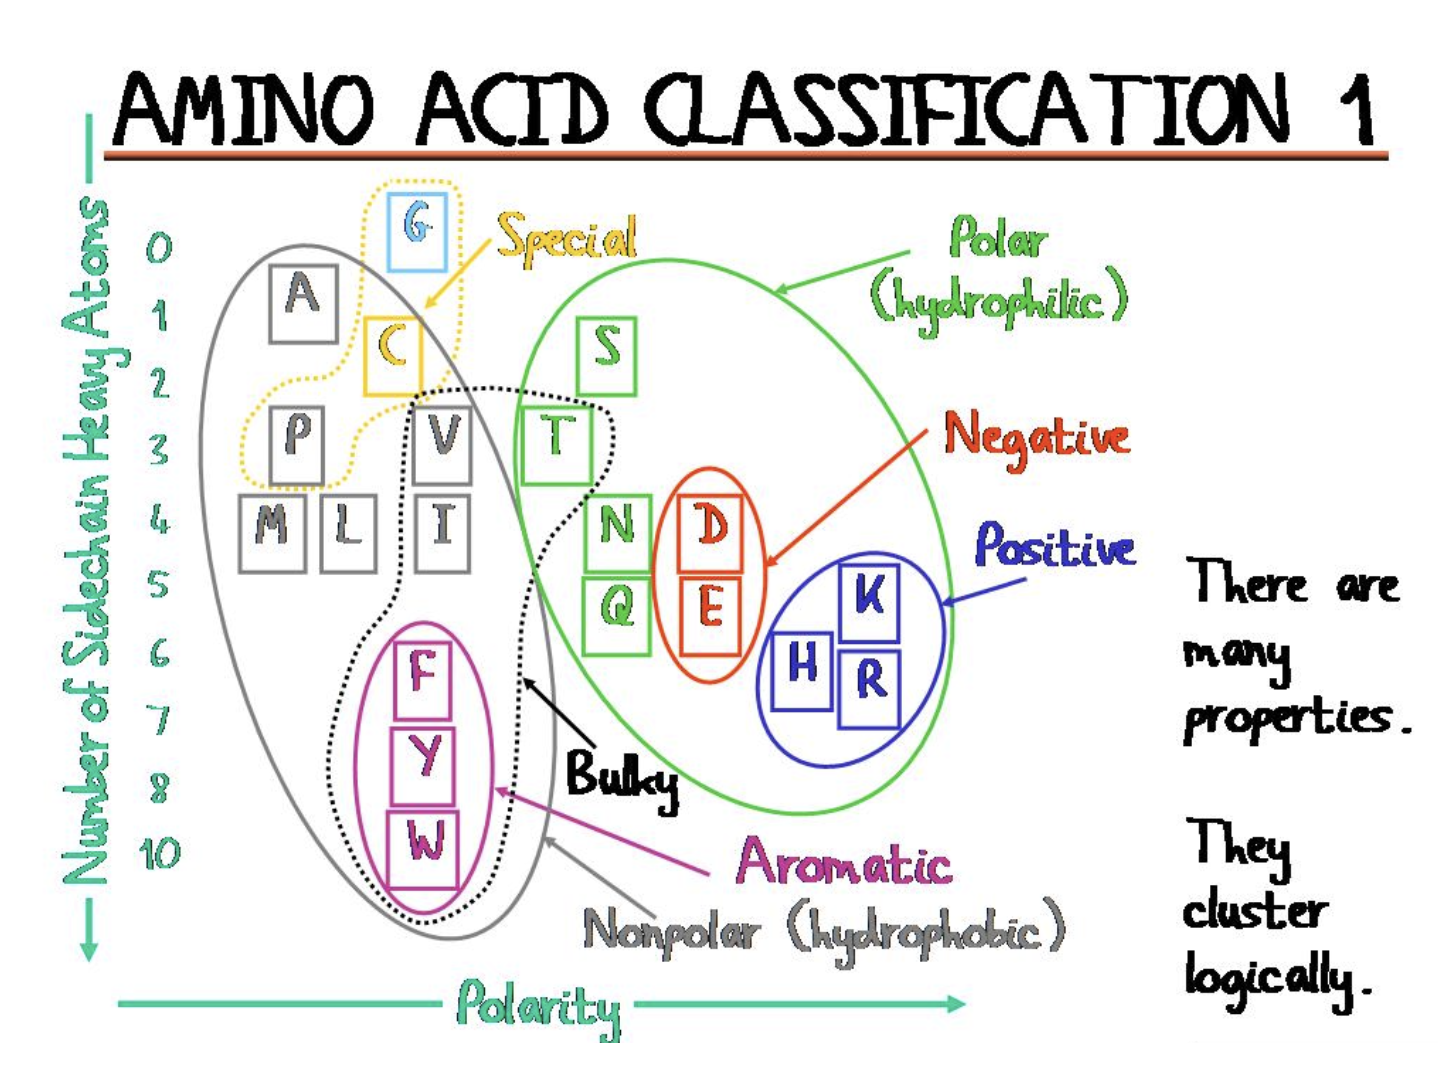
\includegraphics[width =0.8\linewidth]{slides/protein_structure/aminoacid_classification.png}
    \caption*{}
    \label{fig:placeholder}
\end{figure}

\begin{itemize}
    \item So anyway, uh, so what can you expect from this group, for example, which are have a low polarity and have many heavy atoms? What—what do you expect based on the knowledge you have already, let’s say? They would attract many non-polar molecules to themselves. So they would—they would have the compactness, right? You would expect that they would be inside, maybe, of this compact issue, right? 
    \item  And then you can come to here and what you expect, these are the positively charged ones, this is arginine and this is also a ring-containing compound. What do you expect? You expect either that they stay outside because they like water, or you expect that they would create a very specific environment for some reactions and so on, same as for these one. 
    \item And more you go towards kind of medium polarities, you would expect kind of ambiguity, so, you know, behave like this, behave like that, behave like this, behave like that. This kind of things nature like to change something. So these ones, for example, I didn't speak about that much, but it comes, don't worry. These are small residues, serine and threonine, that like to get a phosphate group. So they are small, I just go back for a second that, you know, because I know I'm talking into the air. Serine and Threonine. So two small residues, there's an OH group here, it's called a hydroxyl group. Now, this hydrogen here can be replaced by a phosphate group. Yesterday we had phosphate group, it's P,O,O,O, okay? A big negative charge. This is the kind of the- the mean of- of signaling, communication in between. So they get a phosphate group and then something happens, machine learning will tell probably, okay? But something happens, and then- and then another enzyme comes and takes off the phosphate.
    
    Speaker: So what you need to understand, I mean not- not that heavy biology, but you need to understand some logic. So nature likes regulation, it's very important for complex organisms. It's all about regulation, not about the number of genes, not about the length, not about nothing else, it's about regulation, regulation. Key feature. Okay? Key feature, evolution, adaptation, everything, regulation. So these ones, for example, like to change in a way because they get this post-translational modification, they change and then they make something. For example, they- they pass the signal, they get a phosphate and then the phosphate is taken off.
    
    Speaker: So nature likes this. I'm like this here, I'm like this another place. These are all means of regulation. I get a proton in the cytosol or in the nucleus. You- you start understanding what I'm saying? Okay? Or, you know, so the ones kind of in the middle, it's not what you learn, it's the way how you'll treat them later, okay? You will compute with these very soon.
    
    Speaker: It's all about the changes. These ones change protonation, these ones with the phosphate group we just discussed. Now, these ones are, I- I will- I will talk about them later. These are kind of the neutral versions of these ones. These, for example, are very dangerous, these two. They- they make amyloid aggregates that I explained later, it's more complicated. So, you know, we just created, not we but Michael, we just created a very simple diagram and already you can forecast very important things. So that's the idea of using the grammar, of trying to find a grammar behind some processes, but of course we- we make it much more sophisticated. Just you have to feel the flavor. Okay?

\subsection*{Sequence Complexity predicts Disorder Degree}

\paragraph{An ordered one: Myoglobin}

\begin{figure}[h!]
    \centering
    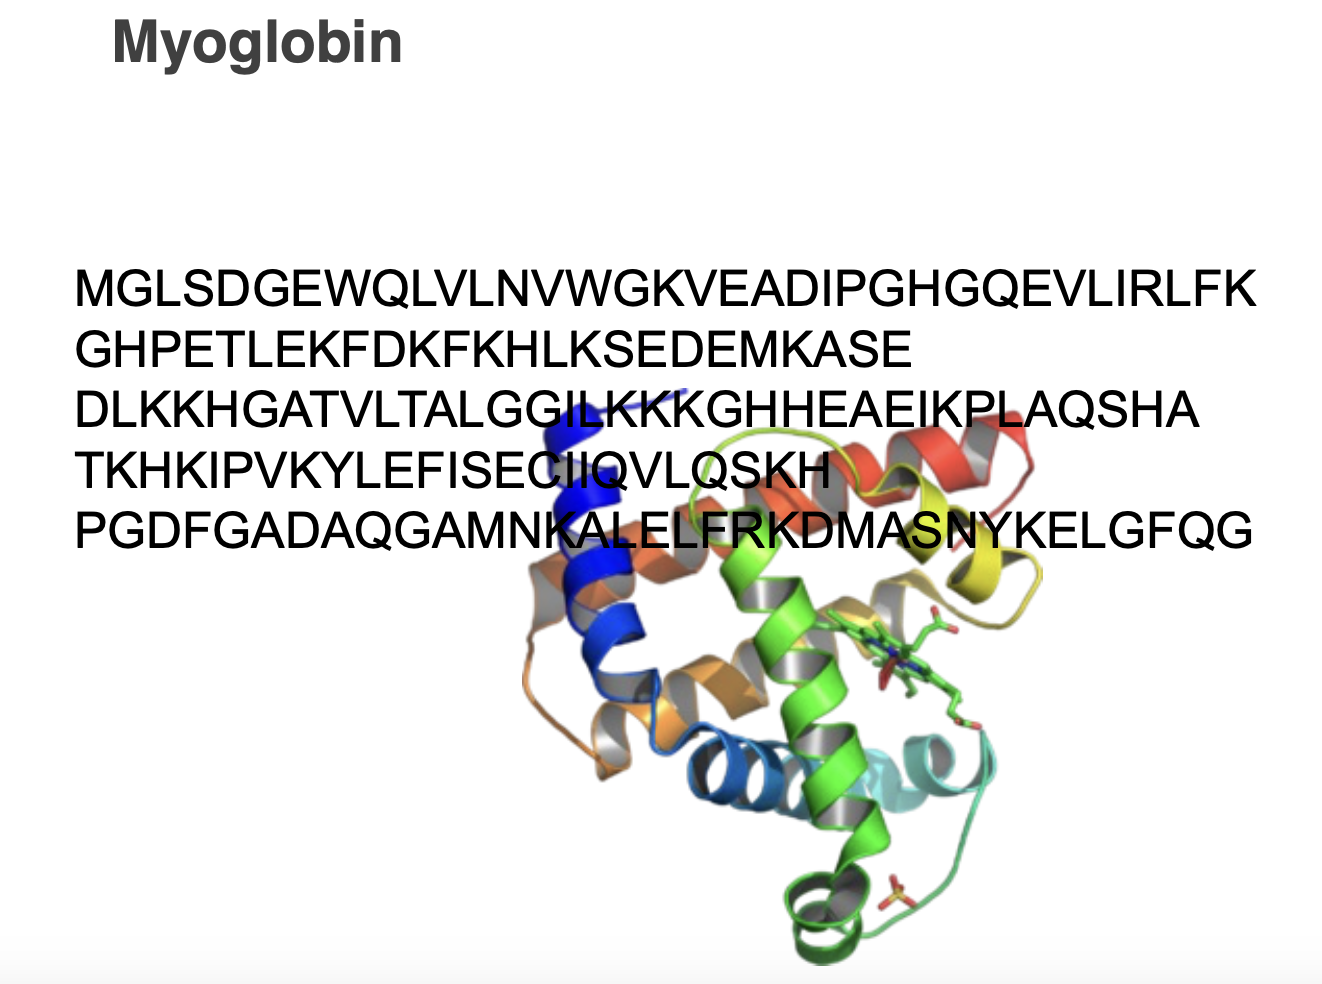
\includegraphics[width =0.8\linewidth]{slides/protein_structure/myoglobin.png}
    \caption*{}
    \label{fig:placeholder}
\end{figure}

There are quite many of these twenty, almost probably all of them are represented here. There are not many repetitions. \textbf{So we can make a conclusion- I mean, it's an early conclusion but- but try to see the- the correlations between things. That if I have many, I have quite nice structure}, so it's- it's quite well defined, even this perpendicularities (between helices) is important, it's- it's quite well defined. 

\paragraph*{A messy one: the Mastermind}

\begin{figure}[h!]
    \centering
    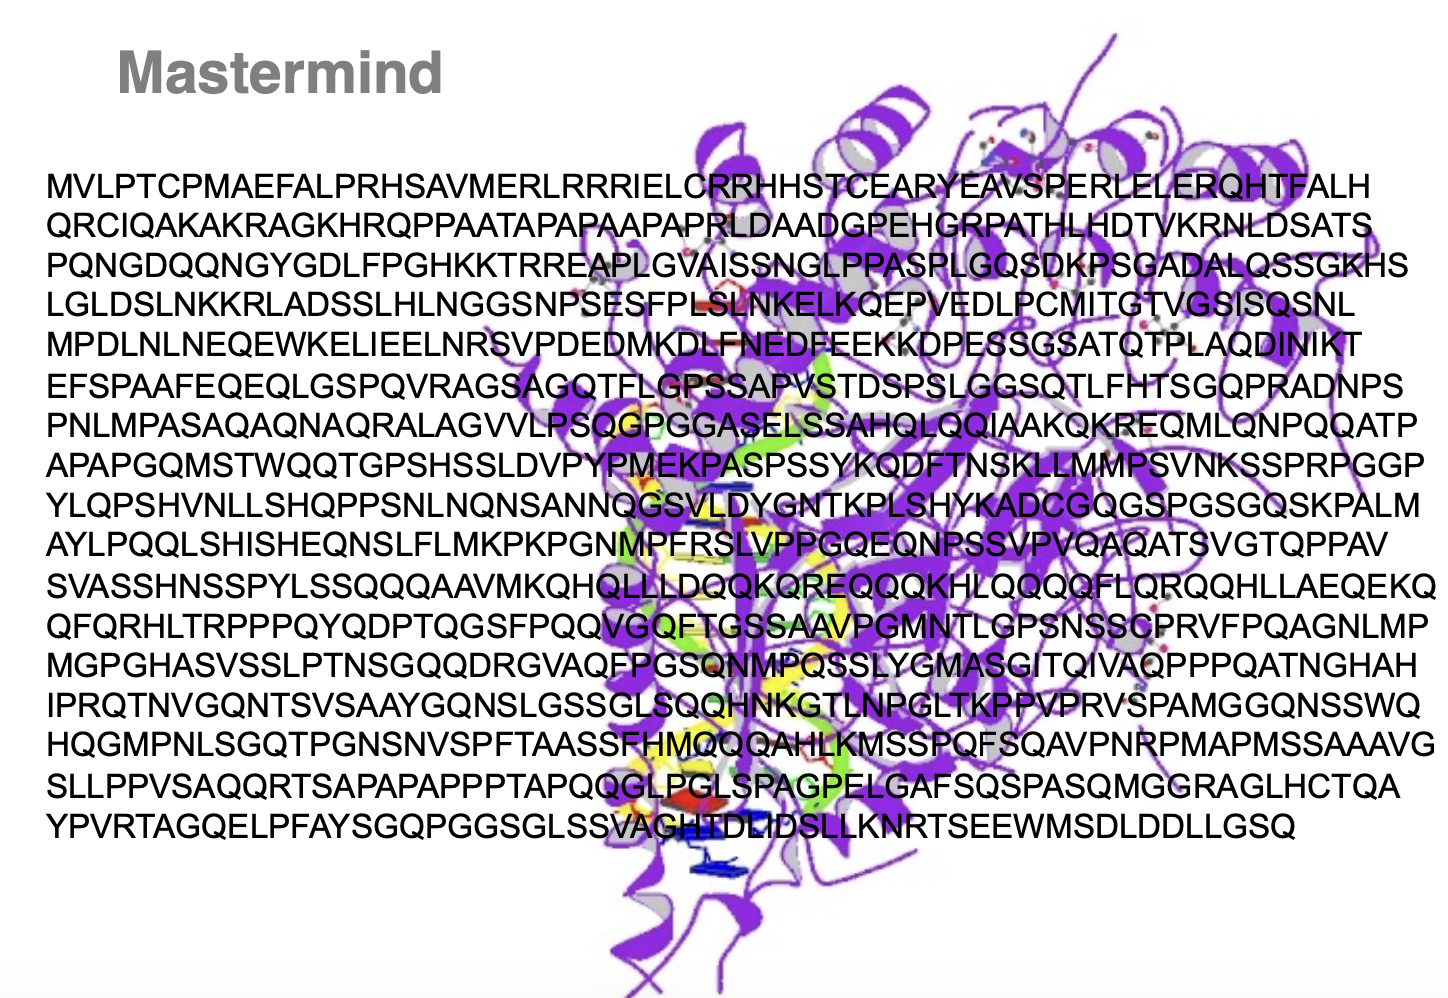
\includegraphics[width =0.8\linewidth]{slides/protein_structure/mastermind.png}
    \caption*{}
    \label{fig:placeholder}
\end{figure}

Now I show you another protein. It's- it's messy basically. Try to read again and tell me something about your reading experience.

Student: There are more repetition in the letters. Repetitions involves different letters

Speaker: Different but not - not any kind, right? That- there are some that are distinguished in this repetition, no? This we note. Like for example, \textbf{G,Q}, \textbf{S,S,S} . And when S is repeated, then many times there is a G there, so there is an associated G. Or if you look, another times there's an associated R.


\paragraph*{A messy one that creates condensates}

One of the key proteins of the ALS disease, the Amyotrophic Lateral Sclerosis. Um, this means you have a single mutation, one amino acid changed, and it starts to grow like a hedgehog. If you don't have a single amino acid mutation, it stays normal like this. 

Speaker: But read the letters. Read the letters. What do you notice?

Student: There are a huge repetitions.

Speaker: What kind of? G,G,G and what else? Q, S... if you look very carefully in the region which I highlighted, if you count how many types of residues are present or dominant, it's different than Myoglobin. I don't know, there are maybe five residues here out of the twenty. So not all the twenty are represented. This is very important. 



\paragraph{High-complexity and Low-Complexity Proteins have very different roles}

\begin{equation}
    H(\text{sequence}) = - \sum_{\small \text{Amino- Acids (AA)}} f_i(AA) \cdot \log_2{f_i(AA)} \quad \textit{Shannon Entropy of a sequence}
\end{equation}

\begin{itemize}
    \item high shannon entropy = high variety of aminoacids. These are called high complexity sequences.
    \item low shannon entropy = low variety of amino-acids. These are called low complexity sequences.    
\end{itemize}

So, does it matter? Of course it does matter, otherwise I wouldn't speak about it. So basically the idea is, if you have a sequence we called high complexity, where the Shannon entropy is high, these are things that are doing reactions, like catalysis. Why? Because in catalysis, you need to place specific groups to specific positions to do a catalysis. And this is very specific, it must be one angstrom away from that one, oxygen, and then the nitrogen must be this- so there is a big constraint, right?  This requires a very complex environment, very high complexity. 



Speaker: Now, what you see on the other side, I hope the video will start, this is so-called, um, pattern specification, or morphogenesis. But this is a very complicated process, and it requires a simultaneous coordination and change in like one thousand processes more or less. So if you put the kind of very strong constraints that you have on the other case, basically you can't- you can't do this. It's not possible. Because if you constrain too much, you- you- there are, you know, you can't coordinate like, I don't know, even hundred processes. But if you have many processes together, evolution can't put a big constraint on one because what happens with the others? 
Speaker: So when there are big constraints, you need a low complexity sequence. Just to achieve. we know exactly which processes are these, we know exactly which proteins are these, and that they are exactly behaving like this. All of them have low complexities.

\paragraph{A sequence could have both low complexity and high complexity domains}

Speaker: So how do you know that this is going to form a droplet and then ages to this hedgehog and then form aggregate? So you want to distinguish these regions. One that will be structured and the other that will not be so structured, or structured only in a case of a pathology. But for example, if you were computing sequence complexities, you should find a great difference in between these two.

\end{itemize}
